\chapter{Experimental Work}

%\section{Technical Approach}

To evaluate the suitability of advanced light transport algorithms to heterogeneous systems, optimized implementations of all algorithms were developed for both \gls{cpu} and \gls{gpu}. These implementations were developed using specialized ray tracing libraries, namely Nvidia Optix \citep{parker2010optix} and Intel Embree \citep{wald2014embree}.


There are two possible schemes of work decomposition across devices. One is image space decomposition, where each device processes a portion of the image pixels. Another possible alternative is to distribute the algorithm iterations across the devices. In \gls{pt} and \gls{bdpt} the choice between these two approaches is almost irrelevant, however in photon based algorithms (\gls{bpm} and \gls{vcm}) it is not that simple. If image plane division was applied, it would force communication between the \gls{cpu} and the \gls{gpu} in every iteration since the photon map, which would be generated concurrently across the devices, has to be shared among them. If an iteration division was applied, for every \gls{cpu} core a complete photon map would be stored in the main memory. When the number of such cores is significant, the memory requirements are too high for most computing systems.

To solve these issues, DICE was configured to consider all the \gls{cpu} cores as a monolithic device, leaving the distribution of work in the \gls{cpu} to the application code. The work between the \gls{cpu} and the \gls{gpu} is then distributed autonomously by the DICE scheduler as a set of independent iterations, eliminating all communication needs. Between the \gls{cpu} cores the image plane is divided, eliminating the excessive memory use. This approach was applied to every developed algorithm in order to ease development and to allow an algorithm independent DICE configuration. The Intel Thread Building Blocks library was used to provide thread parallelism in the \gls{cpu} implementation, due to the ease of use as well as for compatibility with the DICE framework.

%Integrating both \gls{cpu} and \gls{gpu} implementations using DICE was simple, although some adaptations were applied in order to improve efficiency. DICE considers every \gls{cpu} core as an independant device, the same way it considers a \gls{gpu} for the purpose of work sharing. However, for photon mapping based algorithms this is innapropriate because if image plane division was applied, it would force communication between the \gls{cpu} and the \gls{gpu} in every iteration. If an iteration division was applied, for every \gls{cpu} core a complete photon map would be stored in the main memory. In order to solve these issues, DICE was configured to consider all the \gls{cpu} cores as a monolithic device, leaving the distribution of work in the \gls{cpu} to the application code. The work between the \gls{cpu} and the \gls{gpu} is then distributed in a set of independent iterations, eliminationg all communication needs. Between the \gls{cpu} cores the image plane is divided, eliminating the excesive memory use.



\section{Methodology}

To test the scalability and efficiency of the studied algorithms, the execution times of the studied algorithms were measured using only the \gls{gpu}, and while using only the \gls{cpu} or both, with a varying number of \gls{cpu} cores and threads per core, in order to evaluate the gain of using \gls{ht}. Every time measurement was executed five times, selecting the best time as the final result. The workload distribution between the devices was also measured by the DICE scheduler at the end of the five time measurements, being the final result the best possible distribution calculated by DICE. These results represent the fraction of iterations assigned to each device, which may not be a good performance evaluation metric since the iteration time is not uniform, specially in photon mapping based algorithms, in which the iteration time is dependent on the search radius, which decreases in every iteration. These tests were executed using the Living Room Scene with a resolution of 1024x768 and 50 samples per pixel.

To evaluate the image quality produced by the studied algorithms, three scenes were used for testing, each with a different goal. The Sponza scene, courtesy of Crytek, is an outdoor scene with only diffuse materials, but complex geometry nonetheless. The Kitchen scene from Lux Renderer, is an indoor scene with glossy materials. The final and most complex scene, the Living Room, courtesy of Iliyan Georgiev, is an indoor scene as well but with an emphasis on reflected caustics and complex lighting. For every scene a reference image was rendered with \gls{vcm} with 100000 samples per pixel. Then for every algorithm a set of images with an approximate rendering time were produced. All these images were compared to the reference image using the \gls{rmse} metric.


\begin{figure}[H]
\centering
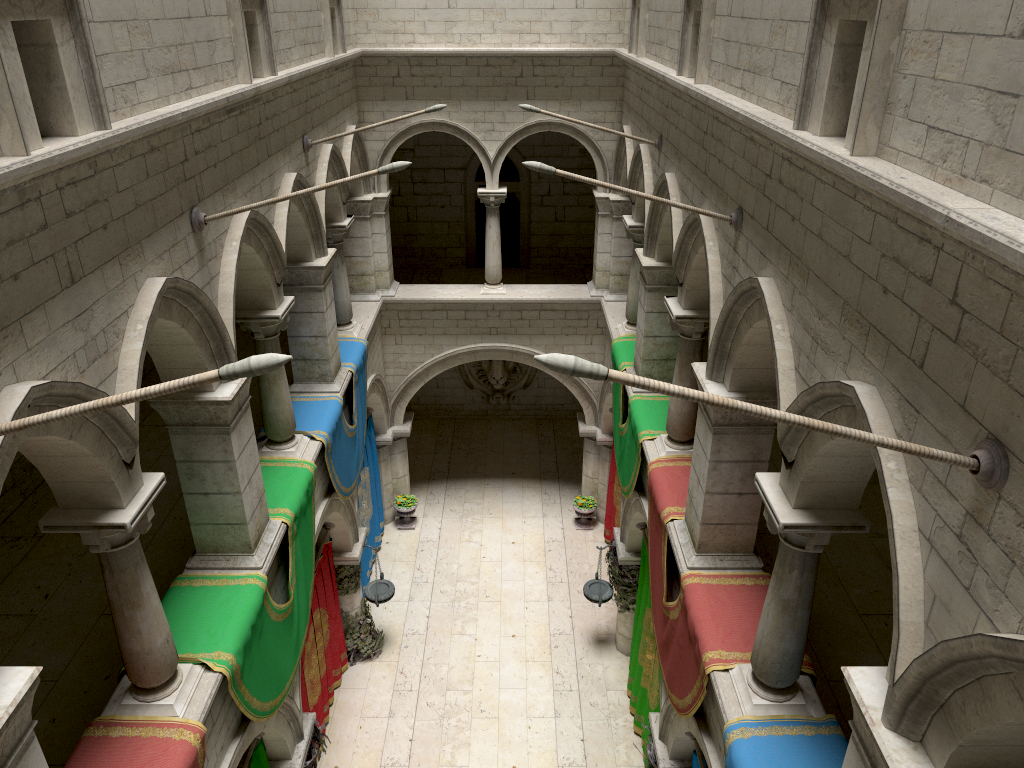
\includegraphics[width=0.8\linewidth]{img/sponza_ref.jpg}
\caption{\label{img:sponza_ref} Sponza scene reference image.}
\end{figure}


\begin{figure}[H]
\centering
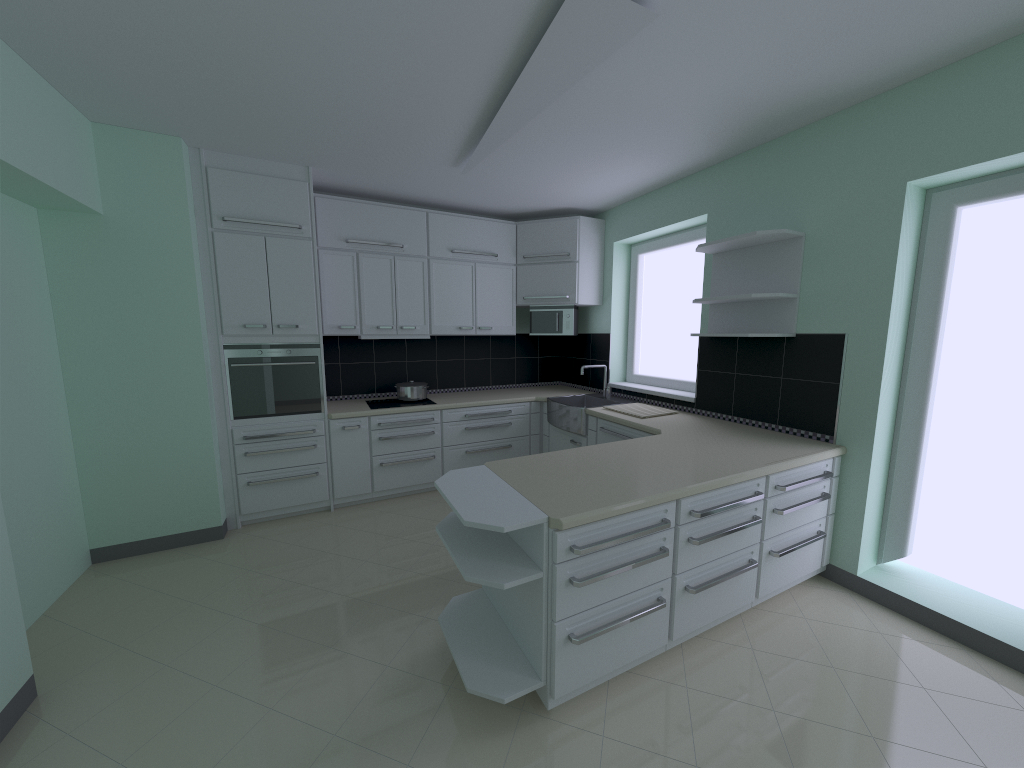
\includegraphics[width=0.8\linewidth]{img/kitchen_ref.jpg}
\caption{\label{img:kitchen_ref} Kitchen scene reference image.}
\end{figure}


\begin{figure}[H]
\centering
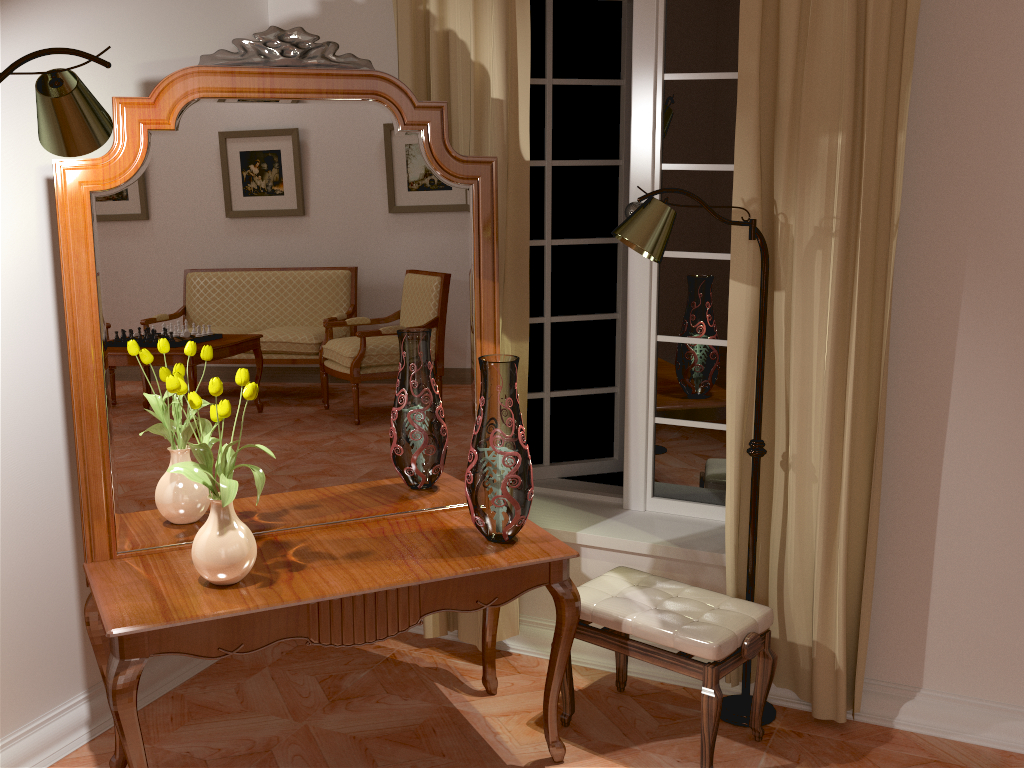
\includegraphics[width=0.8\linewidth]{img/livingroom_ref.jpg}
\caption{\label{img:livingroom_ref} Living Room scene reference image.}
\end{figure}



%\section{Experimental Setup}

All experiments were executed on a dual-socket computer with two 10 core Intel Xeon E5-2670 v2 at the frequency of 2.50 GHz, 64 GB of RAM in a \gls{numa} configuration and a Nvidia Tesla K20 \gls{gpu}.

Every software used was updated to the versions listed in table~\ref{tab:soft_ver}.

\begin{table}[h]
\centering
\begin{tabular}{|l|l|}

\hline
Software & Version \\
\hline
Linux & 2.6.32-279 \\
\hline
GCC & 4.8.2 \\
\hline
CUDA Toolkit & 5.5 \\
\hline
Optix & 3.7 \\
\hline
Embree & 2.5.1 \\
\hline
Intel TBB & 4.3 \\
\hline
\end{tabular}
\caption{\label{tab:soft_ver} Software Used}
\end{table}

\section{Experimental Results}

\subsection{\label{subsec:texec}Execution Time Results}

Figure ~\ref{img:Texec} presents the execution times of the tested algorithms using different device sets. All algorithms show a proportional reduction in execution times with the number of \gls{cpu}'s used. Please note that the "\gls{gpu} only" yellow horizontal line represents a constant value, since no \gls{cpu} cores are used.

\begin{figure}[H]

\centering

\begin{subfigure}[h]{0.45\textwidth}
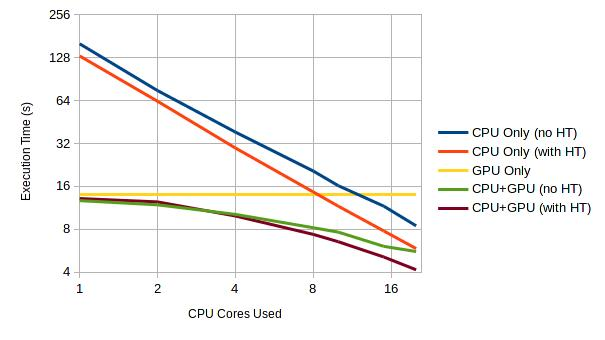
\includegraphics[width=\textwidth]{img/ptTexec.jpg}
\caption{\label{img:ptTexec} PT}
\end{subfigure}
~
\begin{subfigure}[h]{0.45\textwidth}
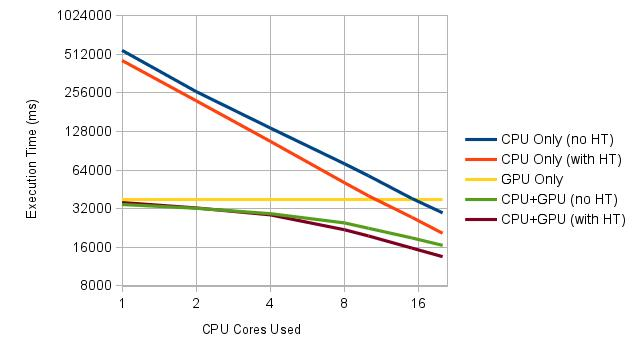
\includegraphics[width=\textwidth]{img/bptTexec.jpg}
\caption{\label{img:bptTexec} BPT}
\end{subfigure}


\begin{subfigure}[h]{0.45\textwidth}
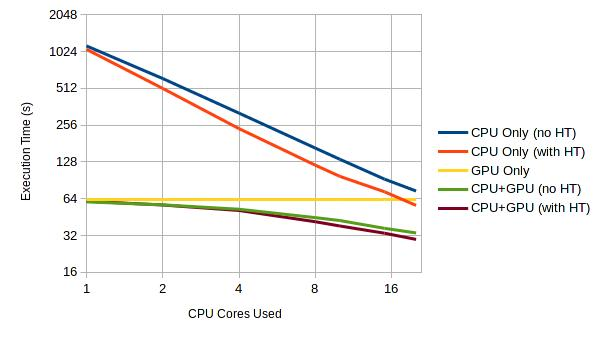
\includegraphics[width=\textwidth]{img/bpmTexec.jpg}
\caption{\label{img:bpmTexec} BPM}
\end{subfigure}
~
\begin{subfigure}[h]{0.45\textwidth}
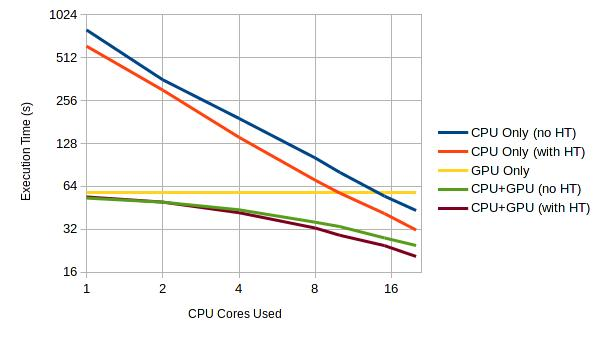
\includegraphics[width=\textwidth]{img/vcmTexec.jpg}
\caption{\label{img:vcmTexec} VCM}
\end{subfigure}

\begin{subfigure}[h]{0.2\textwidth}
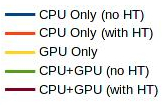
\includegraphics[width=\textwidth]{img/TexecLeg.jpg}
%\caption{\label{img:vcmTexec} VCM}
\end{subfigure}

\caption{\label{img:Texec} Execution Times of the Algorithms}

\end{figure}

\subsection{\label{subsec:cpuspeedup} CPU Speedup Results}

Due to the lack of a clear speedup definition for heterogeneous systems, figure ~\ref{img:speedup} presents only the speedup for the \gls{cpu} implementation. However, in section ~\ref{subsec:hefficiency} there is presented an heterogeneous analysis. Every algorithm achieves an almost linear speedup, with the exception \gls{bpm} that only achieves a speedup of 15.4 using 20 cores. Although not present in this plot, all algorithms take advantage of Hyper Threading, which increases the overall performance between 30\% to 50\%.

\begin{figure}[H]
\centering
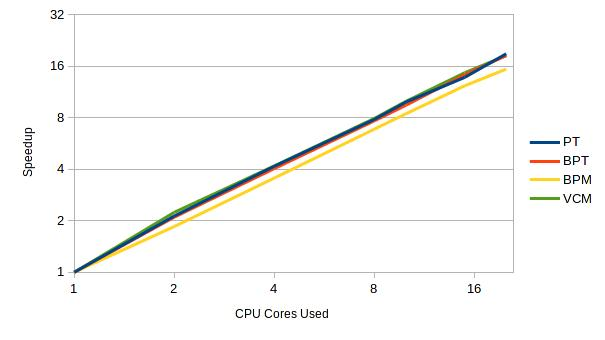
\includegraphics[width=\linewidth]{img/speedup.jpg}
\caption{\label{img:speedup} Speedup Analysis}
\end{figure}

\subsection{\label{subsec:cpuefficiency} CPU Parallelization Efficiency Results}

Due to the lack of a clear efficiency definition for heterogeneous systems, figure ~\ref{img:efficiency} presents only the efficiency for the \gls{cpu} implementation. However, in section ~\ref{subsec:hefficiency} there is presented an heterogeneous analysis. Every algorithm has a parallelization efficiency above 0.9 independently of the number of cores used, except \gls{bpm} that only achieves an efficiency of 0.77 using 20 cores.

\begin{figure}[H]
\centering
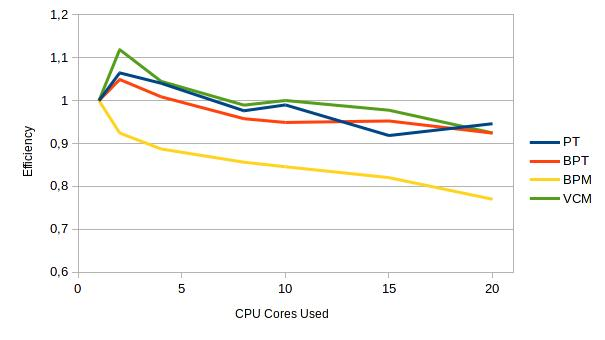
\includegraphics[width=\linewidth]{img/efficiency.jpg}
\caption{\label{img:efficiency} Efficiency Analysis}
\end{figure}

\subsection{\label{subsec:wl} Workload Distribution Results}

Figure ~\ref{img:wl} presents the workload distributions between the \gls{cpu}'s and the \gls{gpu}.  Remember that this is measured as the fraction of iterations processed by each device and that DICE sees the \gls{cpu} as a single device (image space decomposition being then performed among cores by the rendering application itself). The relative workload processed by the \gls{cpu} implementation increases with the number of cores used. This behavior is similar for all four algorithms.

\begin{figure}[H]

\centering

\begin{subfigure}[h]{0.45\textwidth}
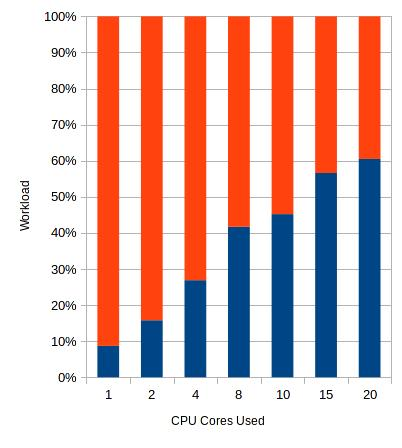
\includegraphics[width=\textwidth]{img/ptwl.jpg}
\caption{\label{img:ptwl} PT}
\end{subfigure}
~
\begin{subfigure}[h]{0.45\textwidth}
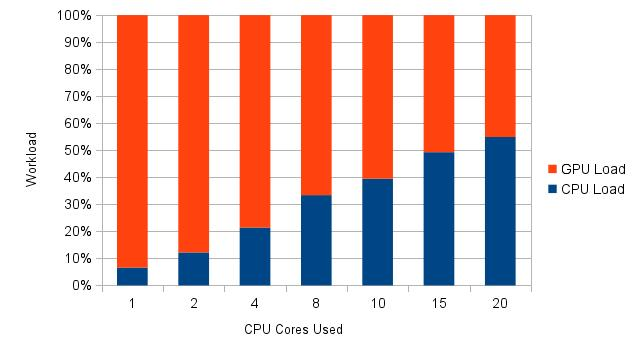
\includegraphics[width=\textwidth]{img/bptwl.jpg}
\caption{\label{img:bptwl} BPT}
\end{subfigure}


\begin{subfigure}[h]{0.45\textwidth}
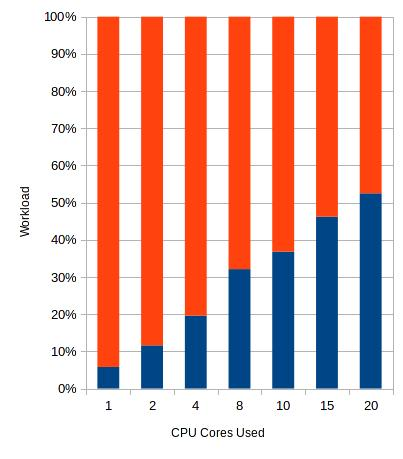
\includegraphics[width=\textwidth]{img/bpmwl.jpg}
\caption{\label{img:bpmwl} BPM}
\end{subfigure}
~
\begin{subfigure}[h]{0.45\textwidth}
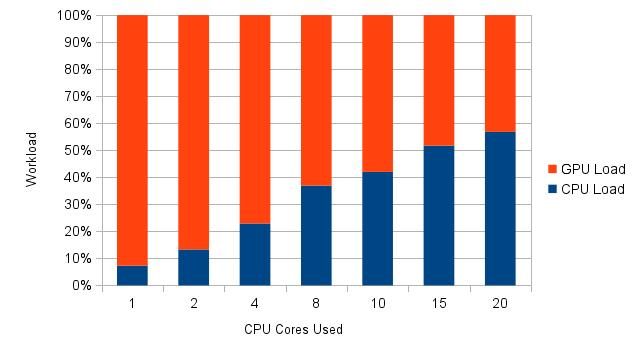
\includegraphics[width=\textwidth]{img/vcmwl.jpg}
\caption{\label{img:vcmwl} VCM}
\end{subfigure}


\begin{subfigure}[h]{0.15\textwidth}
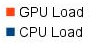
\includegraphics[width=\textwidth]{img/wlLeg.jpg}
\end{subfigure}

\caption{\label{img:wl} Workload Distribution}

\end{figure}

\subsection{\label{subsec:hefficiency} Heterogeneous Efficiency}

%Although all previous metrics seem to indicate that the tested algorithms use all the resources efficiently, there was no absolute measurement of how well the resources were used.

Although all previous metrics may give a notion of how well the heterogeneous implementations have performed, there was no absolute measurement of how well the resources were used.

\cite{Chamberlain98} defined heterogeneous speedup according to equation ~\ref{eq:HetSpeedUp}, where $T_{\mbox{\tiny ref}}$ is the execution time on a reference device selected according to some criterium and $T_D$ is the execution time on an heterogeneous system constituted by the set $D$ of devices.

\begin{equation}
S_h(D) = \frac{T_{\mbox{\tiny ref}}}{T_D}
\label{eq:HetSpeedUp}
\end{equation}

The optimal heterogeneous speedup, $S_h^*(D)$, can not be defined as function of the number of used devices, because different devices offer different amounts of computational power. \cite{Chamberlain98} expressed this ideal speedup as a ratio of computing rates. 

Let the computing rate for the device $d \in D$ for a given workload $W$ be $R_d = \frac{W}{T_d}$, then the ideal computing rate is the sum of all the computing rates of all the devices $d \in D$.

\begin{equation}
R^*_D = \sum_{d \in D} R_d = W \sum_{d \in D} \frac{1}{T_d}
\label{eq:StarCapacity}
\end{equation}

\cite{Chamberlain98} define $S_h^*(D)$ as the ratio between available computing rate and the computing rate of the reference device:

\begin{equation}
S^*_h(D) = \frac{R^*_D}{R_{\mbox{\tiny ref}}} = T_{\mbox{\tiny ref}} \sum_{d \in D} \frac{1}{T_d}
\label{eq:StarHetSpeedUp}
\end{equation}

Given the definitions of heterogeneous speedup and optimal heterogeneous speedup (equations \ref{eq:HetSpeedUp} and \ref{eq:StarHetSpeedUp}), heterogeneous efficiency can thus be defined as the ratio of both

\begin{equation}
E_h(D) = \frac{S_h(D)}{S_h^*(D)} = \frac{R_D}{R^*_D} = \frac{\frac{1}{T_D}}{\sum_{d \in D} \frac{1}{T_d}}
\label{eq:HetEff}
\end{equation}

Given these definitions, it is possible to calculate the efficiency of the heterogeneous implementations using one \gls{gpu} and a varying number of \gls{cpu}'s, as depicted in the figure ~\ref{img:hefficiency}. All algorithms achieve an heterogeneous efficiency above 0.9, except \gls{bpm}.

\begin{figure}[H]
\centering
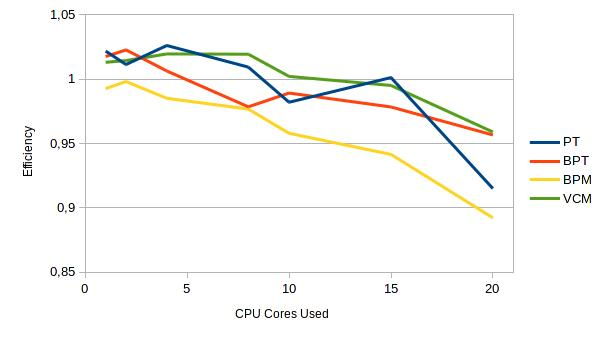
\includegraphics[width=\linewidth]{img/hefficiency.jpg}
\caption{\label{img:hefficiency} Heterogeneous Efficiency Analisys}
\end{figure}


\subsection{\label{subsec:imgq} Image Quality Results}

Figure ~\ref{img:Imgq} presents the image quality measures in function of the rendering time for the various tested algorithms and test scenes.

For Sponza the Path Tracer outperforms the remaining algorithms.

In the Kitchen scene, both Bidirectional Path Tracer and Vertex Connection and Merging algorithms converge to the expected result, although the former is faster for this scene. Both Path tracer and Bidirectional Photon Mapping present lower convergence rates.

In the Living Room scene, Vertex Connection and Merging presents the fastest convergence, while the remaining algorithms converge much more slowly.

\begin{figure}[H]

\centering

\begin{subfigure}[h]{0.45\textwidth}
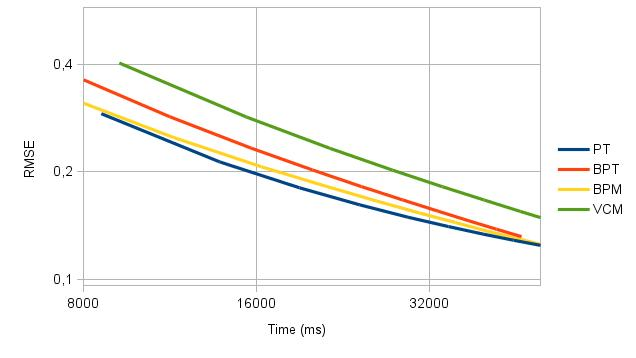
\includegraphics[width=\textwidth]{img/sponzaImgq.jpg}
\caption{\label{img:sponzaImgq} Sponza}
\end{subfigure}
~
\begin{subfigure}[h]{0.45\textwidth}
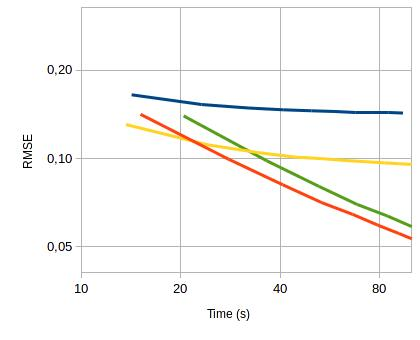
\includegraphics[width=\textwidth]{img/kitchenImgq.jpg}
\caption{\label{img:kitchenImgq} Kitchen}
\end{subfigure}

\begin{subfigure}[h]{0.45\textwidth}
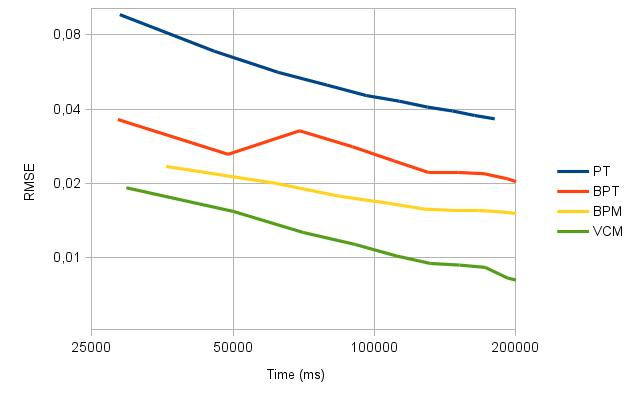
\includegraphics[width=\textwidth]{img/livingroomImgq.jpg}
\caption{\label{img:livingroomImgq} Living Room}
\end{subfigure}
~
\begin{subfigure}[h]{0.1\textwidth}
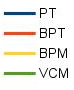
\includegraphics[width=\textwidth]{img/ImgqLeg.jpg}
\end{subfigure}

\caption{\label{img:Imgq} Image Quality Comparison}

\end{figure}

\section{Discussion of Results}

The execution times measures (subsection ~\ref{subsec:texec}) indicate that all algorithms studied are scalable and take advantage of both devices in the rendering process. Note that no inflection point was reached, i.e., a point above which execution time starts increasing with additional processing devices. In fact, all the curves present a negative slope, meaning that not even an horizontal asymptote (i.e., constant execution time with increasing devices) has been reached. This trend suggests that the above referred inflection point is far from being reached and all algorithms should scale well with additional devices. It was not possible to further increase the number of devices in order to detect such inflection point. Speedup and efficiency results (subsections ~\ref{subsec:cpuspeedup} and ~\ref{subsec:cpuefficiency}) also show an almost perfect scalability in the \gls{cpu} implementations, suggesting that the algorithms would scale well for additional \gls{cpu} cores. This hypothesis would have, however, to be verified experimentally.

Previous research \citep{Palhas2013} has shown scalability issues when using the second processor socket in a \gls{numa} architecture with \gls{ppm}. Although with a slightly lower efficiency, the photon mapping based algorithms developed scale across both sockets. This behavior may be due to the usage of specialized ray tracing and threading libraries, such as Embree and Intel Thread building Bocks.

The developed \gls{bpm} implementation has a lower efficiency than all the remaining algorithms. This may be due to the high memory access this algorithm has compared to all the other algorithms, as \gls{bpm} needs to gather lighting from a large number of photons (much more that the photons used in \gls{vcm} and more than the number of vertices accessed by \gls{bdpt} during the connection phase) due to the higher search radius needed to reliably gather photons.

Both workload distribution and heterogeneous efficiency (subsections ~\ref{subsec:wl} and ~\ref{subsec:hefficiency}) results demonstrate that the developed heterogeneous implementation is efficient and that the DICE overhead is minimal and that it always manages to find the optimal workload distribution for every situation in order to maximize the efficiency of the resources used. These results clearly show, for all algorithms, that the workload is distributed among all devices, with the fraction assigned to the \gls{cpu} increasing with the number of cores. This suggests that no devices starve for work, which is a good explanation of why performance scales so well for the number of tested devices. Since these algorithms and the used workload decomposition do not resort to global communications and also do not require work replication across different devices, the other overhead which could be responsible for non-scalable results would be a poor workload distribution; this is clearly not the case. These results are promising in that it makes heterogeneous computing a viable way of reducing the rendering time needed to achieve a given result.

The image quality results (subsection ~\ref{subsec:imgq}) show that each algorithm is best suited for specific situations. In the Sponza scene the best algorithm is Path Tracing due to the outdoor scene configuration, which is detrimental in bidirectional methods due to many of the light paths traced are lost and miss the scene, as well as the simple materials, causing the most relevant light transport paths to be direct illumination and diffuse inter-reflections, which are completely captured by Path Tracing, dispensing with more complex solutions. In the Kitchen scene the best algorithm is the Bidirectional Path Tracing, while Path tracer and Bidirectional Photon Mapping fail to converge at all due to the high variance of the lighting effects present, namely caustics incident on glossy surfaces. In the Living Room scene the Best algorithm is \gls{vcm} due to the presence of many specular-diffuse-specular paths (namely the reflected caustics in the mirror), which \gls{vcm} was specially designed to capture. Although not always the best algorithm, \gls{vcm} is able to converge in every scene (w.r.t. \gls{rmse}), making it the more robust algorithm present among the studied techniques, as shown by previous research \citep{davidovivc2014progressive}.

%As had been shown by all previous performance metrics these four figures clearly show that the algorithms are able to scale as the number of CPU cores increases, demonstrating that all devices are being used. 

%As with \gls{cpu} efficiency, even though it drops with the increase of resources, an inflection point is far from being reached.

\section{DICE Evaluation}

One of the main goal of this work is to evaluate the DICE framework, regarding both performance and usability. After this work, it is possible to say that this framework excels in both points.

Regarding performance, as shown by the previous results (subsections ~\ref{subsec:wl} and ~\ref{subsec:hefficiency}), DICE manages to find the optimal workload distribution for every algorithm and device configuration used, always reaching an heterogeneous efficiency above 85\%. This shows that the framework has a low performance overhead as well as an optimal (or close to optimal) scheduling policy.

Regarding usability, DICE presents to the user a simple and intuitive C++ interface. It was simple to integrate the existing rendering code with DICE due to the possibilities this framework offers regarding how to specify the task to perform: in this work, specialized implementations were passed to the DICE framework. %In order to use DICE, the programmer has only to create a sub-class of the default DICE \verb/work/ class an override the methods \verb/dice/, \verb/estimateWork/ and \verb/execute/, methods that perform the granularity refinement, estimate the portion of work a device executes and execute the given task on the used device. The \verb/execute/ method used in different devices is distinguished by the use of templates.
Other features like the hybrid specification of tasks and the memory manager were not tested.

Overall, DICE proves to be a good solution to take full advantage of heterogeneous systems, being both simple and efficient.